\section{Project organization}
\thispagestyle{plain}
	\subsection{Responsibility Areas}

Good delegation of responsibilities helps so that someone at all times have an overview over what tasks needs to be done in specific areas. This also makes it easier to estimate workloads and delegate tasks during the group meetings. It is important to note that even though there are specific responsibility areas, all the group members will be able to get practical experience in all of the project areas, even though the time spent in different areas will be distributed individually according to the responsobility areas.

\begin{description}
\item[Øyvind Hellenes - Scrummaster] Øyvind was selected as the scrum master because of his leadership qualities and because he early on took an interest in the organizatorial part of the project.
\item[Jon-André Brurberg - Project leader] Jon-André is the driving force in this team and hence, he is also the project leader. Additionally, Jon Andre showed interest in the documentation so he is also responsible for this.
\item[Tor Økland Barstad - Technical coordinator] Tor, with his compentance and knowledge of programming, is our technical coordinator and will thus oversee the code and functions as a technical supervisor for the group.
\item[Jørgen Rugelsjøen Wikdahl - Testing manager] Jørgen is responsible for testing the application to make sure the application has as few bugs as possible.
\item[Hallvard Jore Christensen - Report coordinator] Hallvard have the responsibility of managing the report. This is because of his previous expiriance with report documentation.
\item[Vegard Storm - Usability manager] Vegard showed interest in making sure the application is as user friendly as possible and will manage that aspect of the project.
\end{description}
	
	\subsection{Process model}
For the process model we chose to use the Scrum framework. This was the most natural choice for us amongst the agile methods since it’s a system we all have experience with through previous projects. There are many advantages working with Scrum. It gives clear priority for features and deadlines, which will allow us to focus more of our energy on other vital tasks. This approach promotes communication and transparency. All the team members as well as the client always knows what’s going on and the current tasks’ development through the product backlog. With the backlog cards, the whole production team is also involved with the overall time estimate, which makes it fairly accurate and controllable.

We considered a few other methods as well, like kanban and XP, but came to the conclusion that Scrum was the system for us. This was due to Scrums many structured rules which brings order, but still allows us the freedom we might need during the projects development.

With Scrum we’ll work in iterations called “Sprints” which are typically a week or two, we also stibe towards making these sprints incremental. Doing this, the model is designed, implemented and tested incrementally, feature by feature, until the project is finished. The advantage here is that for every sprint we have a working product to show for, which is a good referance to have, both for ourselves and the customer. 

Since we already have a working project from the very beginning for us to further develop, there is some obvious phase partitions. The first consists mainly on assessing the current version of the product and define the path ahead before we start the actual programming. This will be done through thorough dialog and discussion with SINTEF, to give us a unison idea of where the product are heading. User evaluation is also important in this phase, both internally and externally within the target user group. And of course technology and framework selection. After this comprehensive planning, the actual coding phase can begin. The sprints will be a big part of this, and since we are working incrementally; So we will do with the testing. Following this: the evaluating phase. In which user tests hopefully will force as many problems and bugs with the early version to surface, for us to correct.

Prototypes through a digital mock-up will be important in the planning phase. We have chosen to use Balsamiq for this, which will mean we’ll have an interactive prototype mock-up to show the customer, and should also make sure we're all on the same page. This makes it easier to have something concrete/”physical” as a reference.

\subsection{Development Environment}

Since our project is based on further developing on an existing product, there’s an advantage in using the same main framework as the previous developers. We decided to use Titanium to easily develop a multi-platform app, but we also took a close look at other options (like phonegap) and compared them meticulously in their most critical aspects. With the Titanium framework we use the Titanium SDK which is based on eclipse but tailored for it. For sharing code, Git was our system of choice, mainly because we were already familiar with it, and know it has all the functionality we could need throughout the project. Other documents and files, like notes, summaries, etc. we decided to share through a dedicated Google Drive and Dropbox folder, because each has its own advantages in different aspects. As SCRUM service we first choose Agilefant, but later decided to just use spreadsheets instead.

This project obviously involves working with a big set of APIs, like social media, dictionary and other media services. These’ll play a great part of the development and introduce other frameworks we’ll have to account for. For communication we often use mail and chat-services, but we prefer more “personal” forms of communication like a video chat through skype, phone calls and/or ideally, meetings in person.

\subsection{Work Breakdown Structure}
This Work Breakdown Structure is an overview of what we have done and how our work is distributed between packages. It is updated to match our end result.
We have given percentages to each task to show how much work have been put into it.

\begin{figure}[h!]
\begin{center}
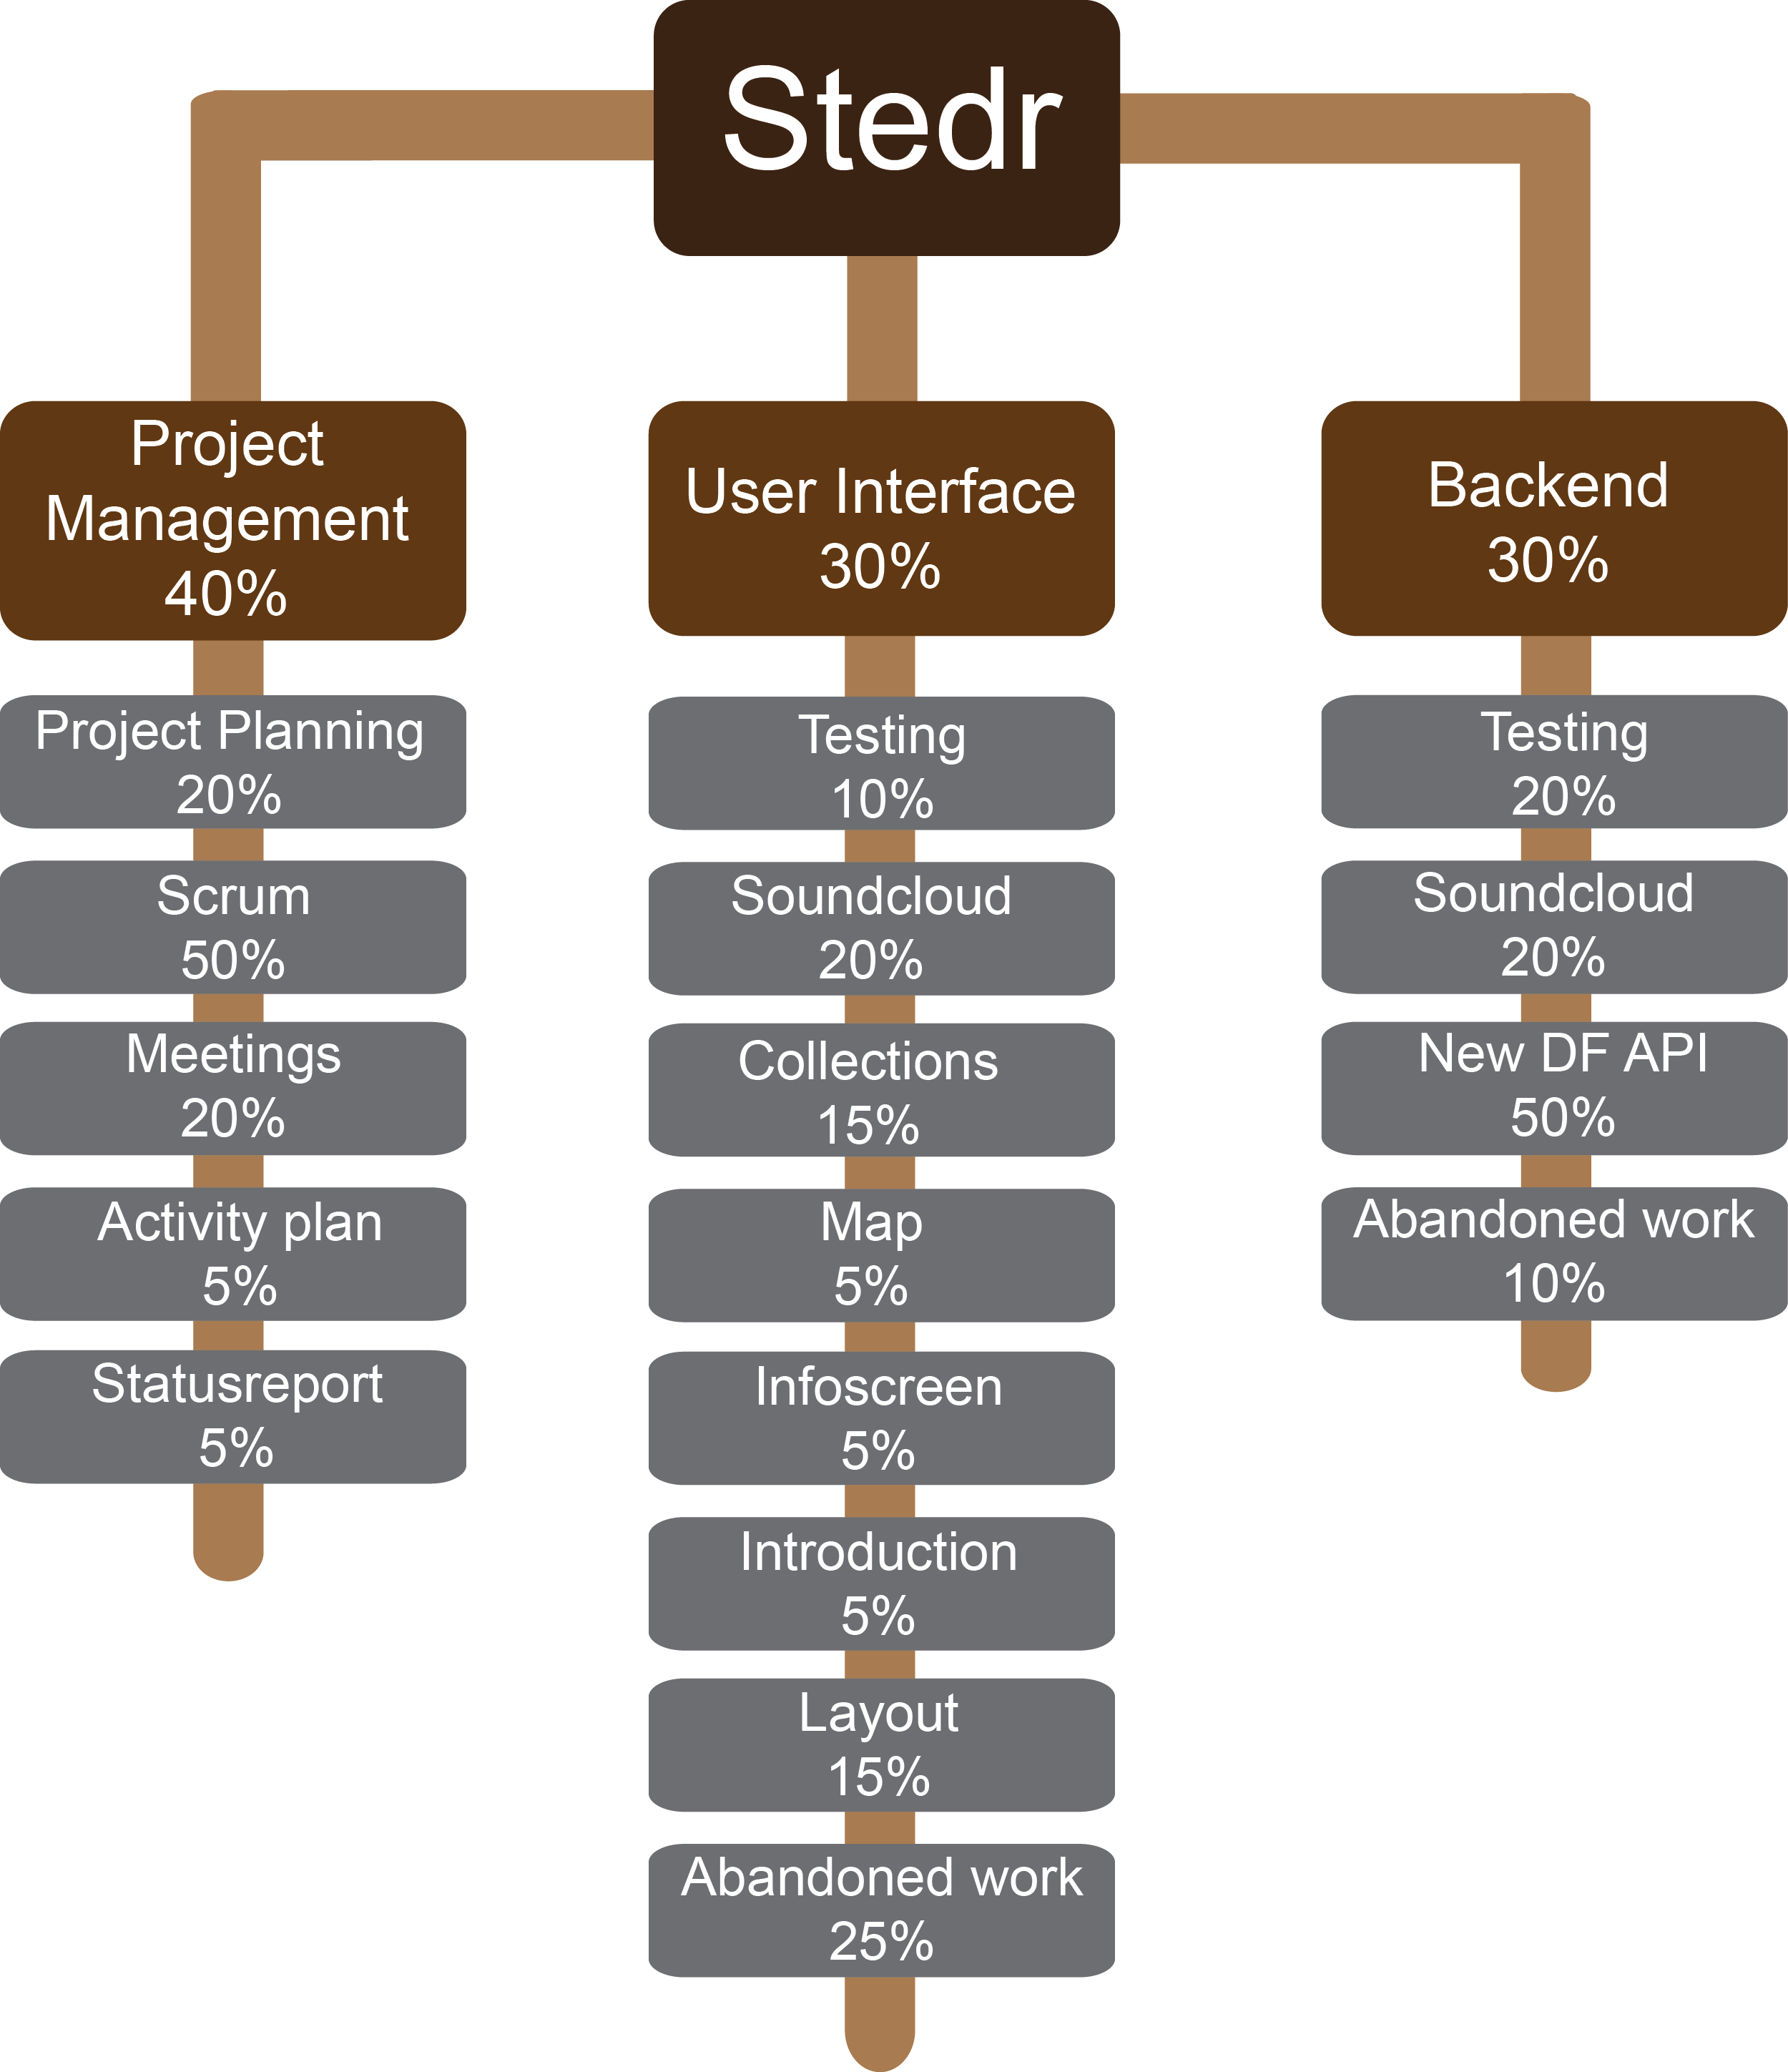
\includegraphics[scale=0.6]{WBS}
\caption{A simple technical overview of the architecture}
\end{center}
\end{figure}
\clearpage

\subsection{Project Planning}


